
% !TeX program = xelatex
% !TEX root = main.tex
% !TeX encoding = UTF-8
\documentclass[10.5pt,compsoc]{CjC}
%\usepackage{CJKutf8}
%\usepackage{CJK}
\usepackage{graphicx}
\usepackage{footmisc}
\usepackage{subfigure}
\usepackage{url}
\usepackage{multirow}
\usepackage[noadjust]{cite}
\usepackage{amsmath,amsthm}
\usepackage{amssymb,amsfonts}
\usepackage{booktabs}
\usepackage{color}
\usepackage{ccaption}
\usepackage{booktabs}
\usepackage{float}
\usepackage{fancyhdr}
\usepackage{caption}
\usepackage{xcolor,stfloats}
\usepackage{comment}
\setcounter{page}{1}
\graphicspath{{figures/}}
\usepackage{cuted}%flushend,
\usepackage{captionhack}
\usepackage{epstopdf}


%===============================%

%\firstfootname{ \quad \quad }
\headevenname{\mbox{\quad} \hfill  \mbox{\zihao{-5}{\songti  计\quad \quad 算\quad \quad 机\quad \quad 学\quad \quad 报 } \hspace {50mm} \mbox{\songti 2024 年 }}}%
\headoddname{\songti
彭渤生, 邢骏洋,王~~京,肖家升:模糊测试技术中测试生成技术综述}%

%footnote use of *
\renewcommand{\thefootnote}{\fnsymbol{footnote}}
\setcounter{footnote}{0}
\renewcommand\footnotelayout{\zihao{5-}}

\newtheoremstyle{mystyle}{0pt}{0pt}{\normalfont}{1em}{\bf}{}{1em}{}
\theoremstyle{mystyle}
\renewcommand\figurename{figure~}
\renewcommand{\thesubfigure}{(\alph{subfigure})}
\newcommand{\upcite}[1]{\textsuperscript{\cite{#1}}}
\renewcommand{\labelenumi}{(\arabic{enumi})}
\newcommand{\tabincell}[2]{\begin{tabular}{@{}#1@{}}#2\end{tabular}}
\newcommand{\abc}{\color{white}\vrule width 2pt}
\makeatletter
\renewcommand{\@biblabel}[1]{[#1]\hfill}
\makeatother
\setlength\parindent{2em}
%\renewcommand{\hth}{\heiti }
%\renewcommand{\htss}{\begin{CJK*}{UTF8}{song}}


\begin{document}
\hyphenpenalty=50000
\makeatletter
\newcommand\mysmall{\@setfontsize\mysmall{7}{9.5}}
\newenvironment{tablehere}
  {\def\@captype{table}}

\let\temp\footnote
\renewcommand \footnote[1]{\temp{\zihao{-5}#1}}


\thispagestyle{plain}%
\thispagestyle{empty}%
\pagestyle{CjCheadings}

\begin{table*}[!t]
\vspace {-13mm}
\begin{tabular}{p{168mm}}
\zihao{5-}
\songti 
计\quad 算\quad 机\quad 学\quad 报\hfill CHINESE JOURNAL OF COMPUTERS\\
\hline\\[-4.5mm]
\hline\end{tabular}

\centering
\vspace{11mm}
\heiti  
{\zihao{2} 模糊测试技术中测试用例生成技术综述 }

\vskip 5mm

{\zihao{3} \fangsong 
彭渤生$^{1)}$\quad  邢骏洋$^{1)}$ \quad 王~~京$^{1)}$ \quad 肖家升$^{1)}$
 }

\vspace{5mm}
\zihao{6}{\songti 
$^{1)}$(南京大学软件学院, 南京, 210093)}

\vskip 5mm
{\centering
\begin{tabular}{p{160mm}}
\zihao{5-}{
\setlength{\baselineskip}{16pt}\selectfont{
\noindent\heiti 摘\quad 要\quad   \songti  

本文综述了模糊测试领域中测试用例生成的研究现状和技术发展。重点分析了基于变异和语法规则的测试用例生成方法,系统梳理了其技术架构演进和最新研究进展。通过对现有技术的评估和总结,文章指出深度学习模型在知识迁移和多模态理解方面的优势将推动模糊测试向更高度智能化和自动化的方向发展,为未来测试用例生成技术的发展提供了新的思路。

 \par}}\\[2mm]

\zihao{5-}{\noindent
\heiti 关键词  \quad \songti  {模糊测试;自动化测试;生成式模糊测试;变异式模糊测试;深度学习  }
 
}\\[2mm]
\zihao{5-}{\heiti 中图法分类号 	\songti  
TP \rm{\quad \quad \quad     }
\heiti DOI号: \songti  
*投稿时不提供DOI号 }
\end{tabular}}

\vskip 7mm

\begin{center}
\zihao{3}{ {\heiti A Survey for Test Generation Techniques in Fuzzing Testing
}}\\
\vspace {5mm}
\zihao{5}{ {\heiti PENG Bo-Sheng$^{1)}$ XING Jun-Yang$^{1)}$ WANG Jing$^{1)}$ XIAO Jia-Sheng$^{1)}$
}}\\
\vspace {2mm}
\zihao{6}{\heiti {$^{1)}$(Software Institute, Nanjing University, Nanjing 210093, China)} }

\end{center}

\begin{tabular}{p{160mm}}
\zihao{5}{
\setlength{\baselineskip}{18pt}\selectfont{
{\bf Abstract}\quad \begin{heiti}
  This paper surveys the current research status and technical developments in test case generation for fuzzing. It focuses on analyzing mutation-based and grammar-based test case generation methods, systematically reviewing their technical architecture evolution and latest research advances. Through evaluation and synthesis of existing technologies, the paper suggests that deep learning models' advantages in knowledge transfer and multimodal understanding will drive fuzzing towards greater intelligence and automation, providing new insights for the future development of test case generation techniques.
\end{heiti}
\par}}\\

\setlength{\baselineskip}{18pt}\selectfont{
\zihao{5}{\noindent 

\vspace {5mm}
{\bf Keywords}\quad \heiti
Fuzzing; Automated Testing; Generation-based Fuzzing; Mutation-based Fuzzing; Deep Learning}\par}
\end{tabular}

\setlength{\tabcolsep}{2pt}
\begin{tabular}{p{0.05cm}p{16.15cm}}
\multicolumn{2}{l}{\rule[4mm]{40mm}{0.1mm}}\\[-3mm]
&\begin{songti}
彭渤生,性别男,2004年生,学位(或目前学历),职称,是/否计算机学会(CCF)会员(提供会员号),主要研究领域为*****、****.E-mail: **************.邢骏洋,性别男,2004年生,本科生,职称,主要研究领域为机器学习、图形化界面软件测试、大语言模型.E-mail: xingjunyang@smail.nju.edu.cn. 王京(通信作者),性别男,xxxx年生,学位(或目前学历),职称,是/否计算机学会(CCF)会员(提供会员号),主要研究领域为*****、****.E-mail: **************.肖家升男,性别,xxxx年生,学位(或目前学历),职称,是/否计算机学会(CCF)会员(提供会员号),主要研究领域为*****、****.E-mail: **************.
第1作者手机号码(投稿时必须提供,以便紧急联系,发表时会删除): … …, E-mail: … …*此部分6号宋体*
\end{songti}
\end{tabular}\end{table*}
\clearpage\clearpage
\begin{strip}
\vspace {-13mm}
\end{strip}
    \linespread{1.15}
\heiti 
\zihao{5}
\vskip 1mm

% 正文内容
\section{引言}
\songti
随着信息化的发展,软件系统的数量、规模和复杂度不断增大。在软件系统的开发过程的,软件测试与漏洞发掘总是至关重要的。遗留的漏洞可能遭受黑客的利用,造成重大的经济损失和信息泄露。例如,2024年7月美国网络安全公司CrowdStrike发布异常更新,导致全球超过850万台Windows设备陷入“蓝屏死机”循环,甚至无法启动。此事件导致银行、航空、电信等多个关键行业的业务中断,重创了包括澳大利亚政府在内的多个组织的基础设施。尽管这一问题迅速被修复,但它揭示了软件更新测试不足和对关键依赖过于集中所带来的高风险\cite{Jones}。另一个例子是2017年的勒索软件WannaCry攻击,这次攻击影响了大约150个国家的约23万至30万台计算机,估计全球经济损失达40至80亿美元。 这次攻击发生的原因是用户没有使用 Microsoft Windows 发布的安全补丁更新他们的系统\cite{Maria}。

为了减少软件漏洞带来的损害,各类软件测试技术蓬勃发展,其中模糊测试已成为当前最流行的方法之一。模糊测试是一种通过随机或半随机的方式生成测试用例,将其输入到目标系统后监听异常结果来发现安全漏洞的安全检测技术。在模糊测试的流程中,输入生成的主要作用是通过不同策略生成能够引发程序异常行为、潜在漏洞或者新代码路径的输入数据。这类样例也被称为“有趣”的样例。确保样例的“有趣”才能保证在后续的测试运行时高效,覆盖率高。从而提高程序的安全性与鲁棒性。

模糊测试输入生成通常遵循以下流程:首先,选择模糊测试目标。可以是源代码、二进制代码,应用程序等。然后必须了解目标接受的输入格式和协议,确保输入数据服务目标预期。生成测试用例时,可以参考之前经过验证的有趣的用例集,或者直接生成新用例。用例的生成策略主要有随机生成和基于语法生成。当测试执行完成之后,对于触发异常的用例,可以保存以供重用或变异后产生新的测试样例。 

基于变异的随机生成测试用例\cite{LibFuzzer, Chenyang, Shuitao}是一种常见的技术,通过注入随机且不可预测的输入来检测应用程序中的漏洞和缺陷。这种方法有助于生成在代码演化或测试阶段尚未探索的新测试用例。然而,随机生成的局限性在于其变异能力的边界限制 - 它只能在现有种子语料库的范围内生成测试用例。如果种子语料库中不包含特定的输入模式或数据结构,就无法生成探索这些特定条件下应用程序行为的测试用例。然而,基于变异的技术可以在更高的抽象级别上操纵输入数据。它可以通过转换输入数据结构(添加/删除)而不是随机更改单个字节来生成新的测试用例。

一个扩展的想法是基于语法生成测试用例\cite{Cornelius, Martin}来为基于生成和变异的模糊测试其提供更好的能力。这种方法利用目标程序接受的输入的形式化语法规范来指导测试用例的生成。通过遵循预定义的语法规则,可以生成在语法上有效的输入,提高测试的效率。与随机生成相比,基于语法的方法能够更好地处理具有复杂输入格式的程序,如编译器、解释器等。此外,将代码片段内联到语法结构中有助于探索代码中的复杂路径,并通过做出使用上下文无关语法无法执行的精确决策来执行复杂操作。但是,它需要对输入语言语法有深入的了解,并且可能需要为复杂或专有的输入语言开发自定义语法。然而,生成的测试用例可能并不总是包含意外或恶意内容,需要进一步变异或生成以增加发现漏洞和错误的可能性。
\vspace {10mm}

\section{基于变异的测试用例生成技术}

\subsection{基础变异策略}

\subsubsection{AFL的经典变异策略及其变种}

AFL(American Fuzzy Lop)作为一个里程碑式的模糊测试工具,其变异策略具有代表性。AFL采用了一种混合变异策略,包括确定性变异和随机变异两种方式。确定性变异(Deterministic Strategy)的含义是指基于一组预定义的规则或模式进行的变异操作,这些操作是可以预测的,这在AFL中主要体现在位翻转(Bit Flip):将输入中的某一位取反,字节翻转(Byte Flip):将输入中的某一个字节取反,算术变异:对输入中的整数进行加减操作,按序插入已知的特殊整数值。

而非确定性变异(Non-Deterministic Strategy)则是指基于随机性的变异操作,这些操作是不可预测的,这在AFL中主要体现在堆叠式位翻转(Stacked bit flips),插入操作(Insertions),删除操作(Deletions),算术运算(Arithmetics),测试用例拼接(Test case splicing)\cite{Zhang}。

AFL同时基于进化算法进行输入队列管理,采用类似自然选择的机制,保留那些能触发新路径的测试用例,通过能量分配机制,优先处理更有潜力的测试用例,定期进行队列精简,去除冗余用例。然而,AFL的变异策略也存在一些局限性,而针对AFL的哈希冲突问题,CollAFL提供了更准确的路径覆盖信息\cite{Collafl},提出了三种变异引导策略:未触及邻居分支引导关注当前执行路径的直接可达区域,未触及邻居后代引导扩展搜索范围到可传递达到的程序区域,内存访问引导特别关注可能导致内存问题的程序位置。

这样一个完整的变异决策体系,不仅提高了变异的精确性,还保持了低开销的插桩。除此之外,对于AFL主要的优化方向包括多种优化方式的集成:在AFL的基础上集成其他先进fuzzer的优化方式,如AFL++\cite{Fioraldi};改进变异策略:例如FairFuzz针对难抵达的分支进行优化,AFLGo专注于获取代码的某些部分的覆盖,PerfFuzz用于查找可能显著减慢程序速度的测试用例,Pythia预测找到新路径的难度,Angora使用新的策略进行变异以增加覆盖范围,Neuzz利用神经网络进行模糊测试;基于QEMU和Unicorn的改进:对于基于QEMU的改进,有TriforceAFL和afl-unicorn等项目,它们允许在QEMU模式下对整个操作系统进行模糊测试\cite{Chang}。

\vspace {10mm}

\subsection{新型变异生成技术}

在模糊测试领域,输入生成的质量和效率直接影响着测试的有效性。传统的模糊测试方法在处理复杂程序时面临诸多挑战:一是难以有效探索深层次的程序路径,特别是那些被复杂约束条件保护的代码分支;二是对于具有特定格式要求的输入,随机变异难以生成符合规范的测试用例;三是在处理魔法数字和嵌套校验和等验证机制时效率低下。早期的研究工作如Miller等人提出的随机字符流注入方法\cite{Miller}以及Sutton等人开发的基于突变的模糊测试框\cite{Sutton},虽然奠定了模糊测试的基础,但在处理结构化输入和复杂程序逻辑时表现出明显的局限性。为了克服这些限制,研究人员提出了多种基于程序分析的新型变异技术。通过引入符号执行、污点分析、梯度下降等技术,新一代的模糊测试工具极大地提升了测试效率和覆盖率。

\vspace{10mm}

\subsubsection{基于程序分析的新型生成技术}
在模糊测试输入生成的评估中,如何提高路径尤其是复杂深层次的路径以及提高测试用例的生成效率是非常重要的参考指标。AFL作为里程碑式的工具通过反馈机制实现了简单易用以及相对高效的随机生成机制。但是AFL仍然存在着复杂和深层次路径难以探索、针对复杂输入格式时难以生成符合规范的输入和路径探索相对随机等问题。在后期发展的各种框架工具中,基于程序分析的符号执行和污点跟踪技术很好的解决了上述问题。

魔法数字和嵌套校验和也是模糊测试中常见的两大难题。魔法数字通常指的是程序中用于验证输入完整性的特定值,而嵌套校验和则涉及到更复杂的数据完整性验证,如在多层数据结构中计算和比较校验和。这些校验机制的存在显著增加了模糊测试的难度,因为随机生成的输入很难通过这些校验,从而导致测试覆盖率降低。为了克服这些难题,研究人员开发了多种技术,包括基于污点分析的方法和基于符号执行的方法,以提高模糊测试的效率和效果。这些技术通过分析程序的行为和输入数据的流向,自动生成能够通过校验的测试用例,从而深入探索程序的状态空间,发现潜在的安全漏洞。

TaintScope\cite{TaintScope}是一个经典的基于动态污点分析和符号执行技术的模糊测试工具,它在无需访问源代码或精确了解平台指令集的情况下,自动检测输入中的校验字段并精确定位程序中的校验基于完整性检查。该工具的主要贡献在于其能够通过控制流修改来绕过这些校验,从而显著提高模糊测试的覆盖率和效率。TaintScope不仅能够识别和绕过校验检查,还能自动修复生成输入中的校验值,使其能够触发潜在的漏洞。这一方法有效地结合了污点跟踪和符号执行的优点。

\begin{figure}[htbp]
  \centerline{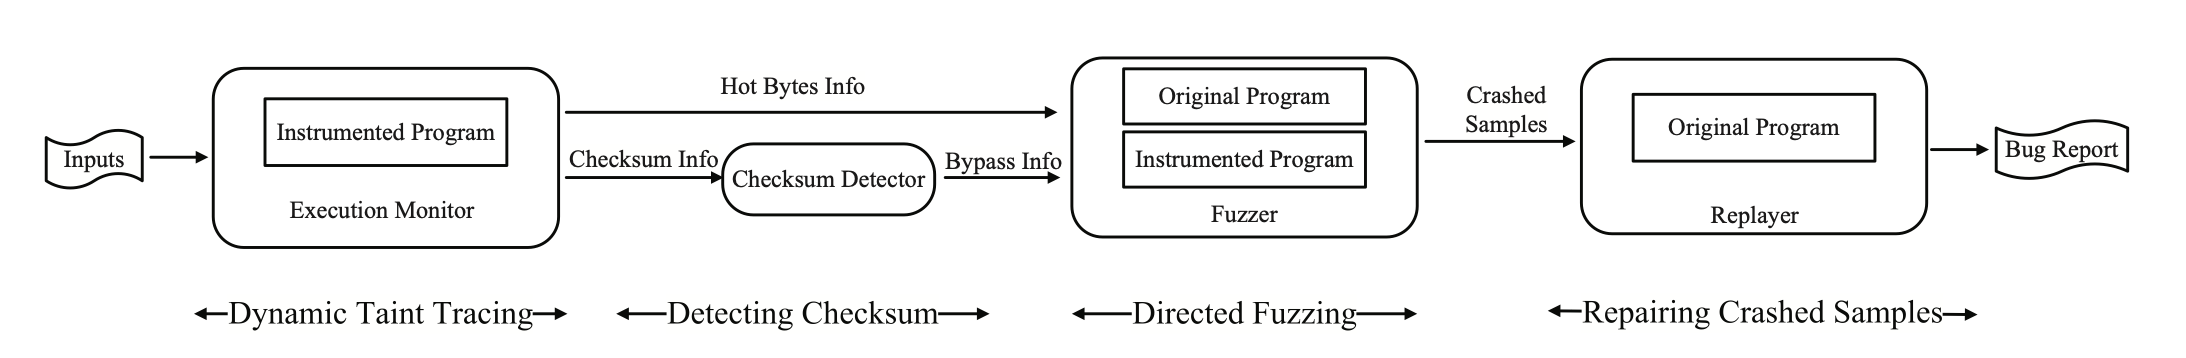
\includegraphics[width=3.15in,height=0.5in]{./image/TaintScope.png}}
  \begin{center}
    图1\quad  TaintScope 系统架构\cite{TaintScope}
  \end{center}
  \label{fig1}
\end{figure}

GreyOne\cite{GREYONE}是一种更先进的数据流敏感模糊测试技术,其关键技术包括轻量级且准确的污点推断FTI、基于污点的输入优先级模型以及约束一致性引导的进化策略。FTI通过监控输入变异时变量值的变化来推断变量的污点状态,这种方法不仅避免了传统污点分析中的劳动密集型工作,而且提高了污点分析的准确性和运行时效率。GreyOne利用FTI提供的污点信息来确定哪些输入字节应该优先变异以及如何变异,以探索更多未触及的代码路径。此外,通过考虑污点变量与未触及分支中预期值的距离(即约束一致性),GreyOne能够调整其进化方向,更有效地探索难以到达的分支。这些技术的结合使得GreyOne在代码覆盖率和漏洞发现方面超越了多种现有的模糊测试工具,展现出其在模糊测试领域的显著优势。

T-Fuzz\cite{T-Fuzz}是另一种基于程序变换的模糊测试方法,它通过移除目标程序中的输入检查来提高代码覆盖率。T-Fuzz利用覆盖引导的模糊测试生成输入,并在模糊测试无法触发新代码路径时,使用轻量级的动态追踪技术检测输入检查,然后将这些检查从目标程序中移除。这种方法允许之前被检查保护的代码被触发,从而有可能发现潜在的错误。T-Fuzz面临的挑战包括移除检查可能导致过度近似和误报,以及在变换程序中触发的崩溃输入可能不会在原始程序中触发错误。为了解决这些问题,T-Fuzz采用了基于符号执行的方法作为辅助的后处理步骤,以过滤掉误报并在原始程序中复现真正的错误。通过变换程序和输入变异,T-Fuzz能够覆盖更多的代码,并发现比现有技术更多的真实错误。

Angora\cite{angora}同样是一种基于变异的模糊测试工具,它通过引入一系列关键技术来提高路径覆盖率,有效解决了路径约束问题。Angora的主要目标是在不使用符号执行的情况下,通过解决路径约束来增加分支覆盖。它采用了可扩展的字节级污点跟踪技术,这种技术通过跟踪输入字节如何流入程序中的每个路径约束,使得Angora能够只变异那些影响路径约束的字节,而不是整个输入,从而大幅减少了探索空间。此外,Angora还采用了基于梯度下降的搜索算法,这种算法在机器学习中非常流行,它避免了昂贵的符号执行,并且能够高效地解决路径约束。Angora还进行了类型和形状推断,这使得梯度下降算法能够更有效地搜索,因为它能够识别输入中哪些字节被集体用作单个值,并推断出这些值的类型。最后,Angora还探索了输入长度,因为某些程序状态只有在输入长度超过某个阈值时才会被探索,而Angora能够检测到这一点并适当增加输入长度。
\vspace {10mm}

\subsubsection{基于输入与程序状态对应关系的新型生成技术}
REDQUEEN\cite{redqueen}是一种新颖的模糊测试方法,它基于输入到状态的对应关系,以提高反馈驱动模糊测试的效率和效果。这种方法特别针对两个常见的模糊测试难题:魔术数字和(嵌套)校验和,这些问题通常需要复杂的程序分析技术,如污点跟踪和符号执行来解决。REDQUEEN通过在程序执行过程中观察输入与程序状态之间的直接对应关系,实现了一种轻量级且高效的解决方案,无需访问源代码或对平台指令集的精确语义。
	与前述两篇论文中提到的Angora和T-Fuzz相比,REDQUEEN在几个关键方面进行了改进和优化。首先,REDQUEEN不依赖于符号执行或污点跟踪,这使得它在大型二进制应用程序和未知环境中更容易扩展且高效。其次,REDQUEEN通过“着色”输入和程序追踪,创建了一种轻量级的污点跟踪近似方法,从而有效地识别和解决魔术数字和校验和问题。此外,REDQUEEN还能够自动修复通过校验和的输入,而无需人工干预或复杂的符号执行方法,这在Angora和T-Fuzz中是不具备的。
  \vspace {10mm}
  
\subsubsection{基于路径感知的新型生成技术}
PATA\cite{PATA}的主要贡献在于其创新性地将路径感知的污点分析技术融入到模糊测试中,显著提升了对复杂软件漏洞的发现能力。传统的模糊测试技术依赖于随机或基于覆盖率的输入变异,而PATA通过精确识别输入数据与程序执行路径中特定变量的依赖关系,实现了对输入数据的智能变异。这种路径感知的污点分析能够区分同一变量在不同执行路径上的多次出现,解决了传统技术在面对循环和多次函数调用时的局限性,从而避免了过污点和欠污点的问题。PATA首先通过构建代表性变量序列(RVS),记录变量在执行路径上的所有出现及其值,然后通过输入微调并匹配RVS来识别影响这些变量值的关键输入字节。这种方法不仅提高了变异的针对性,还增强了模糊测试在探索程序逻辑和发现新漏洞方面的效率。

\begin{figure}[htbp]
\centerline{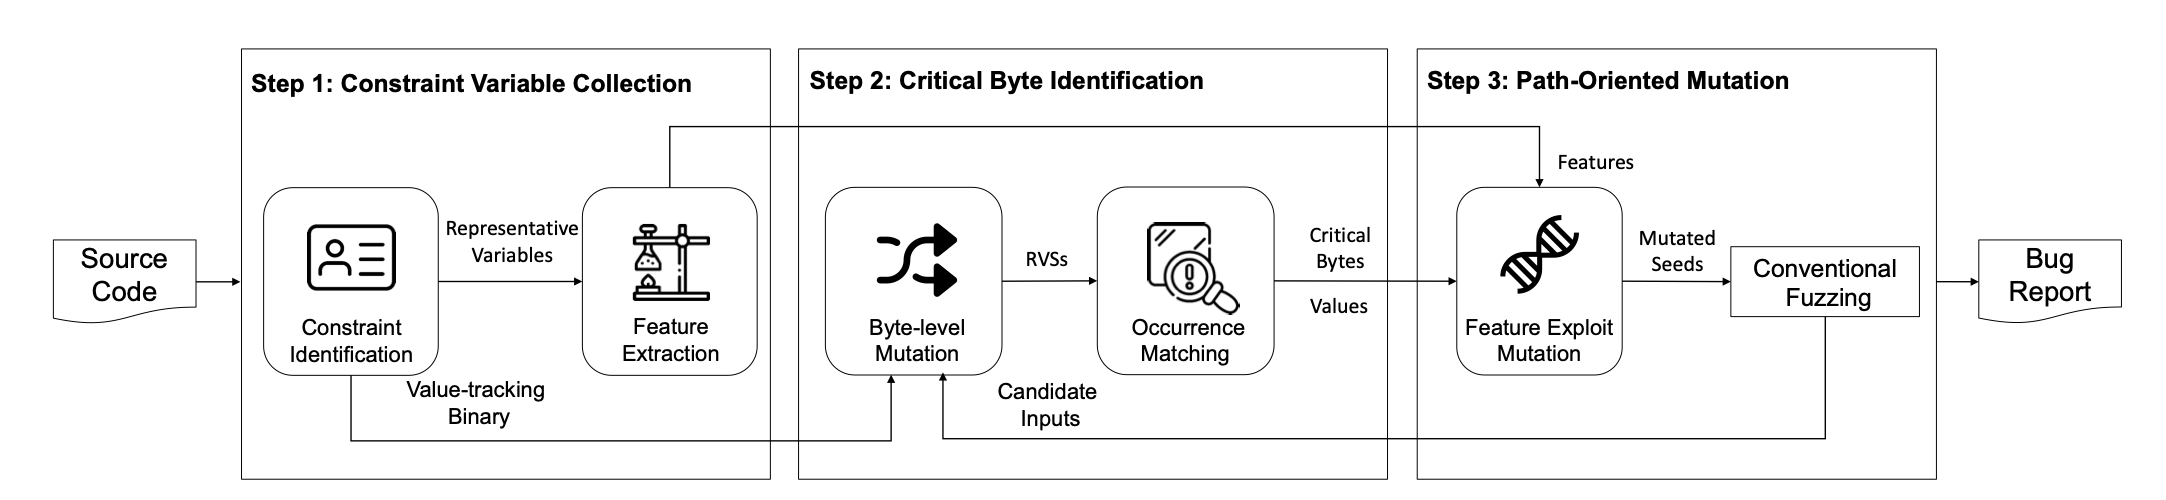
\includegraphics[width=3.15in,height=0.8in]{./image/PATA.png}}
\begin{center}
  图2\quad  PATA整体设计\cite{PATA}
\end{center}
\label{fig2}
\end{figure}

此外,PATA的先进性还体现在其路径导向的变异策略上。利用路径感知污点分析的结果,PATA能够精确地识别出对于每个变量出现至关重要的输入字节,并结合变量的特征和值,选择最合适的变异方法来绕过约束,探索程序状态空间中未被覆盖的分支。这种策略使得PATA在面对复杂的程序逻辑和深层次的漏洞时,能够更加高效地触发新的执行路径和基本块,从而发现更多的独特路径和基本块覆盖。在多个基准测试和真实世界的项目中,PATA相较于现有的先进模糊测试工具,展现出了显著的性能提升,不仅在路径和基本块覆盖上超越了其他工具,而且在漏洞发现方面也表现出色,这进一步证明了PATA在模糊测试领域的创新性和先进性。
\vspace {10mm}

\subsection{定向与智能变异}

在当前软件系统日益复杂的背景下,传统的模糊测试方法往往表现出效率低下和资源浪费等问题。为了解决这个问题,研究人员提出了定向模糊测试和基于机器学习的智能变异方法,试图通过更精准的目标导向和更智能的决策机制来提升测试效果。定向模糊测试通过明确的目标导向,将有限的计算资源集中在最可能存在问题的程序区域,显著提升了测试效率。与此同时,机器学习技术的引入为测试过程带来了全新的智能决策能力,能够从历史数据中学习经验,预测最有价值的测试方向。这两种方法的结合代表了模糊测试技术的未来发展方向,即从"大海捞针"式的随机测试向精准化、智能化的方向演进。

在这一技术背景下,众多研究工作致力于探索如何更好地实现定向测试和智能决策。这些工作在目标识别、路径规划、资源调度等多个方面都取得了重要进展,为提升软件测试的效率和精确度提供了新的思路。

\vspace {10mm}

\subsubsection{定向模糊测试}

定向模糊测试(Directed Fuzzing)是一种有目标性的模糊测试方法,其核心思想是针对程序中特定的代码位置或功能进行测试,通过各种策略引导测试过程到达目标位置,集中资源测试可能存在风险的区域。定向模糊测试主要依靠静态分析确定目标位置,符号执行计算路径约束,动态污点分析跟踪数据流以及启发式算法指导种子选择和变异等技术手段。以DGF为例,它基于模拟退火算法进行功率调度,通过为接近目标位置的种子分配更多能量,同时减少远离目标种子的能量,实现了目标导向的模糊测试。DGF采用模拟退火算法动态调整种子能量,实现全局搜索以覆盖更多目标位置,并支持并行搜索提升效率。它通过计算种子到目标位置的距离来调整能量分配,确保测试资源逐渐向目标位置倾斜。此外,DGF还可以与现有灰盒模糊测试工具(如AFL)集成,利用其轻量级的程序分析和覆盖信息来指导变异过程\cite{Böhme}。

\vspace {10mm}

\subsubsection{机器学习辅助}

机器学习技术正在为模糊测试领域带来革新性的影响。通过对海量测试数据的学习和分析,机器学习能够优化测试过程中的多个关键环节。在种子生成和选择方面,机器学习模型能够预测种子的质量和潜在价值,实现更智能的资源分配。在变异策略上,通过学习历史数据识别最有效的变异模式,提高新执行路径的发现效率。在路径探索方面,机器学习算法能够分析程序结构特征,预测潜在漏洞区域,实现更有针对性的测试。Learn$\&$Fuzz的工作展示了机器学习在测试用例生成中的潜力,它通过无采样预测、概率采样、空间采样和采样模糊等多种策略\cite{Godefroid},结合模型从训练语料中学习到的模式生成多样化的测试用例,同时在特定条件下引入异常以测试错误处理代码。

然而,机器学习辅助的模糊测试也面临获取高质量训练数据困难、实时性要求与推理开销的平衡、模型泛化能力提升以及与传统方法融合等挑战。尽管如此,随着算法和硬件的持续进步,机器学习在模糊测试中的应用前景依然广阔,这种结合必将催生更多创新性的成果。

\vspace {10mm}

\section{基于语法规则的测试用例生成技术}

\subsection{传统的基于语法的测试用例生成技术概述}

传统的基于语法的模糊测试用例生成技术在现代软件测试中扮演着重要角色。与黑盒随机模糊测试和基于约束的白盒模糊测试相比,基于语法的模糊测试在生成有效测试用例方面展现出显著优势。

基于语法的模糊测试的核心在于输入语法的定义。传统上,测试人员根据应用程序需求手动编写语法规则,涵盖数据类型、结构和约束等。然而,这一过程往往繁琐且容易出错,特别是在处理HTML、XML、JSON等复杂的结构化输入时,语法规则的编写需考虑多种情况和边界条件。此外,手动编写的语法规则可能不够全面,导致生成的测试用例无法覆盖所有潜在输入场景,从而影响测试效果。在定义输入语法后,基于语法的模糊测试利用该语法生成测试用例。传统的测试用例生成方法包括随机生成和组合生成:随机生成通过随机选择语法中的词法单元构造输入数据,虽然实现简单,但可能导致生成的测试用例缺乏针对性,无法有效覆盖潜在缺陷;而基于组合生成的方法通过分析语法结构,系统性地组合不同语法元素,生成更为多样化和有效的测试用例。

基于语法的模糊测试在处理复杂结构化输入时,如在网页浏览器、网络协议解析器和数据解析器等领域,展现出了显著优势。这些应用程序往往需要处理”不可信“的输入,如用户提交的HTML、JavaScript代码或网络请求数据等。在这一条件下,基于语法的模糊测试仍能生成符合预期格式的输入,有助于发现潜在的安全漏洞和程序缺陷。

\vspace {10mm}
\subsubsection{输入类型}

基于语法的模糊测试在软件测试中常用的输入类型主要包括结构化输入、边界值输入、特定格式输入和语义输入。结构化输入是基于语法的模糊测试中最常见的输入类型,主要用于处理复杂数据结构的应用,如网络协议解析器、数据解析器和网页浏览器等。这类输入通常通过上下文无关文法(CFG)定义和生成,测试工具根据语法规则构造符合要求的数据。例如,在测试解析JSON数据的应用时,工具根据JSON的语法规则生成合法JSON对象,验证应用的处理能力。

此外,边界值输入关注输入数据的边界情况,如最小值、最大值、空值和超出范围的值等,常用于测试应用程序在处理极端输入时的表现。基于“边界值分析”原则,这种输入类型帮助发现整数溢出、下溢或不当处理等问题。例如,测试一个处理整数的函数时,边界值输入可以包括最大、最小整数及零等,以揭示潜在的逻辑错误和处理漏洞。

另一种特定格式输入是根据应用程序需求生成的输入数据,主要用于测试需要解析特定格式的应用。生成此类输入需要深入分析目标格式,以确保数据符合预定的语法要求。举例来说,在测试网页浏览器解析HTML文档时,特定格式输入可能包括合法的HTML标签和属性,以测试浏览器在解析和渲染时的稳定性与安全性。

语义输入是一种较为高级的输入类型,它不仅符合语法规则,还符合语义上的合理性。生成语义输入需要对应用程序的业务逻辑和语义进行深度分析,以确保模拟真实场景中的用户行为。例如,在测试电子商务网站时,语义输入可能包括合法的产品名称、价格和数量,以测试系统处理这些输入时的反应。语义输入能够更真实地反映用户操作习惯,帮助开发者发现潜在的业务逻辑错误和安全漏洞。与其他类型的输入相比,语义输入在保证符合规则的同时,也能验证应用程序的实际功能和交互合理性。
\vspace {10mm}
\subsubsection{基础理论与方法}

基于语法规则的测试用例生成方法通常依赖于程序或系统的语法描述,结合形式化的语言或模型,自动生成符合预期的输入数据。该方法通常涉及文法模型、语法生成器和语法树构建等关键组成部分。

上下文无关文法(CFG)是形式语言理论中的重要工具,广泛应用于编程语言的定义和自动化测试。CFG通过终结符、非终结符、产生式和开始符号构成,能够清晰地描述编程语言的语法结构。例如,C语言的语法规则可以通过CFG建模,使编译器能够解析源代码并生成相应的抽象语法树(AST)。在模糊测试中,CFG的应用同样重要,研究者们利用CFG生成合法的测试用例,以覆盖程序中的不同代码路径\cite{differential}。例如,FuzzGAN框架中的增强上下文无关文法(enriched CFG)不仅关注语法结构,还引入了额外的语义约束,以确保生成的代码在语法和语义上均有效。这种方法显著提高了生成程序的质量,降低了无效代码的生成概率,从而提升了模糊测试的有效性。

语法生成器是一种自动化工具,旨在根据特定的语法规则生成合法的程序或输入数据。它在编程语言的设计与实现中扮演着关键角色,尤其在编译器构建和模糊测试应用中。通过利用CFG,语法生成器能够生成符合语言语法规范的代码,为程序的验证和测试提供支持。在模糊测试中,语法生成器通过遵循特定的语法规则生成合理的测试输入,从而提高测试的覆盖率和有效性。如在FuzzGAN框架中,研究者利用生成对抗网络(GAN)结合语法生成器,自动生成符合C语言语法的测试用例。这种方法不仅提高了测试用例的质量,还能够有效识别编译器中的潜在错误和漏洞。

语法树构建是编译器设计和程序分析中的重要环节,将源代码转换为结构化的表示形式,即抽象语法树(AST)。AST有效反映程序的语法层次和逻辑关系,为后续的语义分析、优化和代码生成提供支持。构建AST的过程包括词法分析和语法分析,前者将源代码分解为词法单元,后者则利用CFG对词法单元进行解析,检查其是否符合语言的语法规则。在模糊测试中,语法树构建同样发挥着重要作用:生成合法的AST使得模糊测试工具能够自动生成符合特定语法的测试用例,从而提高测试的有效性和覆盖率。例如,DEEPFUZZ框架通过训练生成模型,学习原始测试数据中的语法模式,生成新的合法程序,覆盖更多的代码路径,有助于发现潜在的缺陷和安全漏洞。
\vspace {10mm}
\subsection{基于学习的新型生成技术}

随着深度学习和人工智能技术的不断发展,基于学习的测试用例生成方法逐渐成为模糊测试领域的重要研究方向。相比传统的随机生成或规则驱动的方法,这些方法通过学习输入数据的特征和规律,自动生成更加智能、精准的测试用例,能够有效提升测试覆盖率和测试质量。基于学习的生成技术不仅能够应对复杂系统中的多样性和高维度问题,还能根据应用上下文和输入数据的分布进行智能化的测试用例设计,从而更好地发现程序中潜在的缺陷和漏洞。

Zest是一种创新的基于语法的测试用例生成方法\cite{zest},该技术首先将类似QuickCheck的随机输入生成器转化为确定性参数生成器,通过这种转化,Zest能够将一系列未类型化的比特(称为“参数”)映射为语法合法的输入。这一过程强调了对输入生成的精确控制,确保生成的输入不仅符合特定的语法规则,还能为后续的测试分析,特别是语义分析阶段,提供有效的测试用例。Zest的核心在于采用突变策略引导生成新的测试输入,这与覆盖引导模糊测试(Coverage-guided fuzzing, CGF)的方法相似。通过在比特层面进行突变操作,Zest能够引发语法合法的结构突变,从而有效探索更复杂的语法结构,增强代码的覆盖率。与传统的随机输入生成方法相比,Zest提供了一种更高效且定向的测试用例生成方式,确保输入的语法合法性,避免了生成无效输入的常见问题。Zest专注于生成能够触发语义分析阶段错误的有效输入,提升了测试的深度与广度。

DeepFuzz是一种自动化的语法基础模糊测试工具,旨在持续生成符合语法的C程序,以有效测试生产编译器\cite{DeepFuzz}。具体而言,DeepFuzz能够生成具有不同复杂度和功能的程序,包括简单的函数调用、条件语句和循环结构,这种多样性有助于全面测试编译器的处理能力。此外,DeepFuzz在输入生成过程中采用预处理步骤,去除注释、统一空白字符并合理处理宏定义,确保生成程序的风格一致性和语法正确性,避免因格式不一致或语法错误导致的测试失败。同时,DeepFuzz通过对生成程序的自动验证,确保其在语法上有效,进一步提高了测试的可靠性。最后,DeepFuzz的输入生成技术具有高效性和可扩展性,通过并行化生成过程,能够快速生成大量测试用例,显著缩短模糊测试的时间,其生成模型可根据不同测试需求进行调整和扩展,以适应不同编译器和程序特征。这种灵活性使DeepFuzz能够在多种环境下有效应用,提升编译器的稳定性和安全性。

\begin{figure}[htbp]
  \centerline{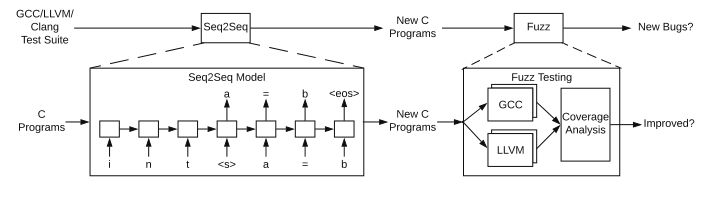
\includegraphics[width=3.15in,height=1.2in]{./image/DeepFuzz.png}}
  \begin{center}
    图3\quad  DeepFuzz 系统架构\cite{DeepFuzz}
  \end{center}
  \label{fig1}
\end{figure}

现今的研究将深度学习模型引入到模糊测试中,通过学习大量的输入数据,生成更加智能、精准的测试用例,提升测试的效率和效果。这些技术在模糊测试领域展现出了强大的潜力,有望成为未来软件测试的重要发展方向。

FuzzGAN是一种基于生成对抗网络(GAN)的创新模糊测试框架\cite{FuzzGAN},旨在增强深度神经网络(DNN)在对抗性输入下的鲁棒性。该框架通过生成模型与判别模型的对抗训练机制,专注于生成多样化且具有挑战性的测试用例,以有效检测DNN中的潜在脆弱性。FuzzGAN的输入生成技术具有显著优势,首先通过训练生成模型学习原始输入数据的分布,从而合成符合该分布的样本。这种方法不仅确保生成的测试用例在语法和语义上与原始输入相似,还能捕捉数据中的复杂特征和模式,提升测试用例的有效性和多样性。与传统的基于突变的模糊测试方法相比,FuzzGAN生成的输入不再局限于简单变换,而是能够生成更加复杂和多样的对抗样本,从而更全面地评估DNN的鲁棒性。

CAGFuzz是一种针对图像基础深度学习系统的覆盖引导对抗生成模糊测试方法\cite{CAGFuzz},旨在提升深度神经网络(DNN)模型的测试效率和准确性。该方法通过引入覆盖引导的模糊测试技术,结合对抗样本生成,克服了传统对抗生成方法在迁移性和深层特征提取方面的不足。CAGFuzz的核心在于其输入生成技术,具体包括基于一般数据集训练的对抗样本生成器(AEG),该生成器不仅考虑了数据特征,还通过余弦相似度约束确保生成的对抗样本在深层特征上保持一致性,从而有效提高了对抗样本的迁移性。其输入生成过程具有显著优势,能够生成针对主流DNN模型的对抗样本,揭示潜在的错误和缺陷。同时,通过深层特征的提取与分析,CAGFuzz确保生成的对抗样本不仅在表面上类似于原始样本,而且在语义上保持一致性,这使得其在模型重训练时能够显著提高准确性。

Automatic Text Input Generation自动文本输入生成技术能够自动生成与应用上下文相关的有效文本输入\cite{atigmt}。该方法的核心是利用深度学习模型,特别是递归神经网络(RNN),通过对大量已记录的输入数据进行训练,学习输入与应用上下文之间的关联。具体而言,RNN模型能够捕捉到用户输入的语义和上下文信息,从而在测试过程中生成与当前操作环境相匹配的文本输入。例如,在一个搜索类应用中,当用户点击搜索框时,系统可以自动生成相关的搜索关键词,而不是随机生成无意义的字符,这样不仅提高了测试的有效性,还能确保测试流程的顺利进行。通过这种方式,自动文本输入生成技术能够有效地推动测试进程,使得测试工具能够深入到应用的复杂工作流中,执行更为全面的测试。

Zest、FuzzGAN、CAGFuzz、DeepFuzz和Automatic Text Input Generation这些技术通过结合深度学习、生成对抗网络、语法分析等多种方法,在模糊测试用例生成中展现出了强大的能力。

\vspace{10mm}

\subsection{基于语法规则的新型生成技术}

基于语法规则的生成技术通过利用程序语言的语法特性,自动生成符合特定语法规则的输入数据。与传统的随机生成或人工编写测试用例的方法不同,基于语法的生成方法能够在保证输入合法性的同时,探索更广泛的代码路径和潜在漏洞。

Grammatical Category Objects(GCO)技术是通过将上下文无关文法转换为Java类,以实现自动化测试数据的生成\cite{Beyene}。该方法的核心在于利用语法的结构特征,生成符合特定格式的字符串,从而有效地测试软件在处理这些字符串时的正确性和鲁棒性。GCO技术的实施过程首先涉及对上下文无关文法的解析与转换,生成相应的Java类(称为Grammatical Category Objects)。这些类不仅能够表示语法规则,还可以通过实例化生成符合语法的字符串。通过这种方式,GCO技术能够生成多种多样的测试用例,从而覆盖软件中的不同代码路径,提高代码覆盖率。研究表明,GCO技术在生成测试用例时,可以与其他测试方法相结合,例如一致性测试套件和启发式算法,以进一步提升测试的全面性和有效性。具体而言,GCO技术能够有效地生成深层语法树的字符串,这对于测试复杂的语法结构尤为重要。通过这种方式,测试人员能够确保生成的字符串不仅符合语法规则,还能够触发软件中可能存在的边界情况和潜在缺陷。此外,GCO技术还能够通过深度优先搜索等确定性方法,探索生成所有可能字符串的空间,从而实现对语法规则的全面覆盖。

Evolutionary Generative Fuzzing是一种基于进化生成的模糊测试技术\cite{Evo},旨在有效发现Kotlin编译器中的潜在缺陷。该技术的核心在于创新的输入生成方法:其结合了语法特征建模和进化算法,以生成多样化的测试用例,从而全面评估编译器的功能和性能。具体而言,该模糊测试技术通过构建Kotlin语言的语义和语法模型,利用增强的上下文无关文法(CFG)生成符合Kotlin语法的随机代码片段,确保生成的输入程序在语法上有效,反映Kotlin语言的复杂特性。此外,研究者们引入基于遗传算法的输入生成策略,通过自然选择和遗传变异机制,推动生成过程朝向更为多样化和复杂的代码。这种进化方法不仅提高了生成程序的多样性,还有效覆盖了不同的语言特性,增强了模糊测试的有效性。

Skyfire是一种创新的数据驱动种子生成方法,旨在为处理高度结构化输入的模糊测试程序生成高质量的种子输入\cite{Skyfire}。它比上述两种方法作用更为广泛。该方法通过利用大量样本自动提取语法和语义规则的知识,从而生成分布均匀的种子输入。Skyfire与基于变异的模糊测试方法是互补的,能够为这些方法提供高质量的种子输入,进而提升它们在处理高度结构化输入时的效率和有效性。

需要注意的是,前述如EGF等方法能通过语义丰富的文法产生上下文感知的代码片段,以减少无效代码的生成。然而,对于多数用例生成方法,如何在生成代码时平衡语法与语义,确保生成的代码不仅符合语法规则,还能触发有意义的语义问题,仍是一个挑战。以CLP(约束逻辑编程)为例,尽管CLP能够有效地平衡语法与语义,生成具有特定语法特征和语义行为的程序,但不同编程语言的多样性使得生成过程十分复杂\cite{Dewey}。例如,强类型静态语言(如Scala)和弱类型静态语言(如C)具有不同的类型系统和内存模型,这要求生成工具能够分别处理这些特定语言的特性。另外,由于语言规范和实际实现之间常常存在差异,某些被认为是缺陷的问题可能并不被开发者视为语言错误。以typechecker fuzzing为例,部分开发者认为某些类型约束的处理方式虽然违反了类型系统的某些理论规范,但从实际编译器实现角度来看,并不算真正的错误\cite{Dewey}。这种不一致性使得测试用例生成技术不仅要关注规范的精确性,还需要考虑开发者对语言行为的接受度。

\vspace{10mm}


\section{总结与展望}

在模糊测试领域,生成式和变异式测试用例生成方法正朝着与人工智能技术深度融合的方向发展。深度学习模型,尤其是大型预训练模型,以其卓越的代码理解和生成能力,为模糊测试技术的创新开辟了新路径。首先,这些模型通过学习海量程序代码,能够深入理解程序的语义结构、控制流程和数据依赖关系,从而帮助生成式测试方法突破传统基于语法规则的局限。它们能够自动推断程序的输入约束和边界条件,生成符合程序预期的高质量测试用例,减少对人工定义语法规则的依赖。

同时,深度学习模型的知识迁移能力使得在不同程序间共享和复用测试经验成为可能,这对于提高测试效率具有重要意义。对于变异式测试方法,深度学习模型可以通过分析历史测试数据和程序执行轨迹,学习到更智能的变异策略。它们能够预测哪些变异操作更可能产生有价值的测试用例,优化变异过程中的决策,尤其是在处理复杂的数据结构和协议时。

随着深度学习技术的不断进步,未来的模糊测试将更加智能化和自动化。模型可以自适应不同类型的程序和输入格式,动态调整测试策略。在处理具有复杂约束的程序时,模型可以结合符号执行和动态分析技术,更精确地解决路径约束问题。此外,大模型强大的多模态理解能力也使得它可以处理更多样化的输入类型,如图形界面、网络协议等。

然而,在应用深度学习技术时也需要注意几个关键问题:首先是模型的可解释性,需要确保测试过程的可控性和结果的可理解性;其次是计算资源的平衡,需要在模型的复杂度和实用性之间找到适当的平衡点;最后是测试的完整性和可靠性,需要确保基于模型的测试方法能够维持较高的代码覆盖率和漏洞发现能力。

未来,模糊测试技术可能会朝着"混合智能"的方向发展,将传统的测试技术与新兴的人工智能方法有机结合。这种结合不仅包括深度学习模型的应用,还可能涉及强化学习、知识图谱等技术,形成更完善的测试生态系统。通过持续学习和优化,这样的系统能够不断提升测试效率和准确性,为软件安全性保障提供更有力的支持。同时,随着大模型技术的发展,模糊测试也可能实现更高层次的智能化,如自动理解软件需求、自动生成测试策略、自动修复发现的漏洞等,从而推动软件测试领域向更高水平发展。

\begin{strip}
\end{strip}

% 参考文献、致谢、附录、作者简介
\vspace {3mm}
\zihao{5}{
\noindent \heiti 致\quad 谢 \quad  \kaishu}
感谢软件学院的房春荣老师和助教们,为本文提供了很多帮助,并为我们的综述写作提供了入门级的指导。

感谢YZW,在我们紧张的时候带来了很多欢乐。

\vspace {5mm}
\centerline
{\zihao{5}
\heiti 参~考~文~献 }

\begin{thebibliography}{99}
\zihao{5-}
\vspace{3mm}
	\bibitem{Jones}
  Jones, J. (2024, July 19). A 'blue screen of death loop': How a Crowdstrike update crashed Microsoft systems around the world. City AM. Retrieved from https://www.cityam.com
	\bibitem{Maria}
	 Maria F. Prevezianou. 2021. WannaCry as a Creeping Crisis. Springer International Publishing.
  \bibitem{LibFuzzer}
  LibFuzzer 2017. libFuzzer—A Library for Coverage-guided Fuzz Testing. Retrieved from https://llvm.org/docs/LibFuzzer.html
  \bibitem{Chenyang}
  Chenyang Lyu, Shouling Ji, Chao Zhang, Yuwei Li, Wei-Han Lee, Yu Song, and Raheem Beyah. 2019. MOPT: Optimized mutation scheduling for fuzzers. In Proceedings of the 28th USENIX Security Symposium, 1949–1966.
  \bibitem{Shuitao}
  Shuitao Gan, Chao Zhang, Peng Chen, Bodong Zhao, Xiaojun Qin, Dong Wu, and Zuoning Chen. 2020. GREYONE:
Data flow sensitive fuzzing. In Proceedings of the 29th USENIX Security Symposium, 2577–2594.
  \bibitem{Cornelius}
  Cornelius Aschermann, Tommaso Frassetto, Thorsten Holz, Patrick Jauernig, A.-R. Sadeghi, and Daniel Teuchert. 2019. NAUTILUS: Fishing for deep bugs with grammars. In Proceedings of the Network and Distributed System Security
Symposium (NDSS’19). 1–15.
  \bibitem{Martin}
  Martin Eberlein, Yannic Noller, Thomas Vogel, and Lars Grunske. 2020. Evolutionary grammar-based fuzzing. In Proceedings of the 12th International Symposium of Search-Based Software Engineering (SSBSE’20). Springer-Verlag, 105–120.
  \bibitem{Zhang}
  Zhang, S. (n.d.). Technical "whitepaper" for afl-fuzz. Retrieved from http://lcamtuf.coredump.cx/afl/
  \bibitem{Collafl}
  Gan, S., Zhang, C., Qin, X., Tu, X., Li, K., Pei, Z., and Chen, Z. (2018, May). Collafl: Path sensitive fuzzing. In 2018 IEEE Symposium on Security and Privacy (SP) (pp. 679-696). IEEE.
  \bibitem{Fioraldi}
  Fioraldi, A., Maier, D., Eißfeldt, H., and Heuse, M. (2020). {AFL++}: Combining incremental steps of fuzzing research. In 14th USENIX Workshop on Offensive Technologies (WOOT 20).
  \bibitem{Chang}
  Chang, Z. (2019, April 29). AFL 及其相关拓展项目总结. 
  \url{https://zanderchang.github.io/2019/04/29/AFL%E5%8F%8A%E5%85%B6%E7%9B%B8%E5%85%B3%E6%8B%93%E5%B1%95%E9%A1%B9%E7%9B%AE%E6%80%BB%E7%BB%93/}
  \bibitem{Miller}
  Miller, B. P., Fredriksen, L., and So, B. (1990). An empirical study of the reliability of UNIX utilities. Communications of the ACM, 33(12), 32-44. https://doi.org/10.1145/96267.9627
  \bibitem{Sutton}
  Sutton, M., Greene, A., and Amini, P. (2007). Fuzzing: Brute Force Vulnerability Discovery. Addison-Wesley Professional. ISBN:978-0-321-44611-4
  \bibitem{TaintScope}
  Wang, T., Wei, T., Gu, G., and Zou, W. (2010). TaintScope: A Checksum-Aware Directed Fuzzing Tool for Automatic Software Vulnerability Detection. In Proceedings of the 2010 IEEE Symposium on Security and Privacy (SP'10). https://doi.org/10.1109/SP.2010.37
  \bibitem{GREYONE}
  Gan, S., Zhang, C., Qin, X., Wu, D., Zhao, B., Qin, X., and Chen, Z. (2020). GREYONE: Data Flow Sensitive Fuzzing. In Proceedings of the 29th USENIX Security Symposium (12-14 August 2020). USENIX Association. 
  \url{https://www.usenix.org/conference/usenixsecurity20/presentation/gan}
  \bibitem{T-Fuzz}
  Peng, H., Shoshitaishvili, Y., and Payer, M. (2018). T-Fuzz: Fuzzing by Program Transformation. In 2018 IEEE Symposium on Security and Privacy (SP'18). https://doi.org/10.1109/SP.2018.00056
  \bibitem{angora}
  Chen, P., and Chen, H. (2018). Angora: Efficient Fuzzing by Principled Search. 2018 IEEE Symposium on Security and Privacy, 711-714. DOI: 10.1109/SP.2018.00046x`'
  \bibitem{redqueen}
  Aschermann, C., Schumilo, S., Blazytko, T., Gawlik, R., and Holz, T. (2019). REDQUEEN: Fuzzing with Input-to-State Correspondence. In Network and Distributed System Security (NDSS) Symposium (24-27 February 2019). San Diego, CA, USA. https://dx.doi.org/10.14722/ndss.2019.23371
  \bibitem{PATA}
  Liang, J., Wang, M., Zhou, C., Wu, Z., Jiang, Y., Liu, J., Liu, Z., and Sun, J. (2022). PATA: Fuzzing with Path-Aware Taint Analysis. In 2022 IEEE Symposium on Security and Privacy (SP)
  \bibitem{Böhme}
  Böhme, M., Pham, V.-T., Nguyen, M.-D., and Roychoudhury, A. (2017). Directed Greybox Fuzzing. In Proceedings of the 2017 ACM SIGSAC Conference on Computer and Communications Security (CCS ’17). Dallas, TX, USA: Association for Computing Machinery. https://doi.org/10.1145/3133956.3134020
  \bibitem{Godefroid}
  Godefroid, P., Peleg, H., and Singh, R. (2017). Learn$\&$Fuzz: Machine Learning for Input Fuzzing. In Proceedings of the 32nd IEEE/ACM International Conference on Automated Software Engineering (ASE 2017). Urbana-Champaign, IL, USA: IEEE. 978-1-5386-2684-9/17
  \bibitem{differential}
  Liu, J., Huang, Y., Wang, Z., Ma, L., Fang, C., Gu, M., Zhang, X., and Chen, Z. (2024). Generation-based differential fuzzing for deep learning libraries. *ACM Transactions on Software Engineering and Methodology, 33*(2), Article 50. https://doi.org/10.1145/3628159 
  \bibitem{zest}
  Padhye, R., Lemieux, C., Sen, K., Papadakis, M., and Le Traon, Y. (2019). Semantic fuzzing with Zest. *Proceedings of the 28th ACM SIGSOFT International Symposium on Software Testing and Analysis (ISSTA '19)*, 329-340. https://doi.org/10.1145/3293882.3330576
  \bibitem{DeepFuzz}
  Liu, X., Li, X., Prajapati, R., and Wu, D. (2019). DeepFuzz: Automatic generation of syntax valid C programs for fuzz testing. In *Proceedings of the Thirty-Third AAAI Conference on Artificial Intelligence / Thirty-First Innovative Applications of Artificial Intelligence Conference / Ninth AAAI Symposium on Educational Advances in Artificial Intelligence* (pp. 1044-1051). AAAI.
  \bibitem{FuzzGAN}
  Han, G., Li, Z., Tang, P., Hu, C., and Guo, S. (2022). FuzzGAN: A generation-based fuzzing framework for testing deep neural networks. In *Proceedings of the 2022 IEEE 24th International Conference on High Performance Computing $\&$ Communications; 8th International Conference on Data Science $\&$ Systems; 20th International Conference on Smart City; 8th International Conference on Dependability in Sensor, Cloud $\&$ Big Data Systems $\&$ Applications* (pp. 1601-1608). IEEE. https://doi.org/10.1109/HPCC-DSS-SmartCity-DependSys57074.2022.00244
  \bibitem{CAGFuzz}
  Zhang, P., Ren, B., Dong, H., and Dai, Q. (2022). CAGFuzz: Coverage-guided adversarial generative fuzzing testing for image-based deep learning systems. *IEEE Transactions on Software Engineering, 48*(11), 4630-4646. https://doi.org/10.1109/TSE.2021.3124006
  \bibitem{atigmt}
  Liu, P., Zhang, X., Pistoia, M., Zheng, Y., Marques, M., and Zeng, L. (2017). Automatic text input generation for mobile testing. In *Proceedings of the 39th International Conference on Software Engineering (ICSE)* (pp. 643-653). IEEE. https://doi.org/10.1109/ICSE.2017.65
  \bibitem{Beyene}
  Beyene, M., and Andrews, J. H. (2012). Generating string test data for code coverage. In *Proceedings of the 2012 IEEE Fifth International Conference on Software Testing, Verification and Validation* (pp. 395-404). IEEE. https://doi.org/10.1109/ICST.2012.107
  \bibitem{Evo}
  Georgescu, C., Olsthoorn, M., Derakhshanfar, P., Akhin, M., and Panichella, A. (2024). Evolutionary generative fuzzing for differential testing of the Kotlin compiler. In M. D'Amorim (Ed.), *Companion Proceedings of the 32nd ACM International Conference on the Foundations of Software Engineering, FSE Companion 2024* (pp. 197-207). ACM. https://doi.org/10.1145/3663529.3663864
  \bibitem{Skyfire}
  Wang, J. J., Chen, B. H., Wei, L., and Liu, Y. (2017). Skyfire: Data-driven seed generation for fuzzing. In *Proceedings of the 38th IEEE Symposium on Security and Privacy (SP)* (pp. 579-594). IEEE. https://doi.org/10.1109/SP.2017.23
  \bibitem{Dewey}
  Dewey, K., Roesch, J., and Hardekopf, B. (2015). Fuzzing the Rust typechecker using CLP (T). *Proceedings of the 30th IEEE/ACM International Conference on Automated Software Engineering (ASE)*, 482-493. https://doi.org/10.1109/ASE.2015.65

\end{thebibliography}

\clearpage\clearpage

\begin{strip}
\end{strip}

\begin{biography}[pbs.jpg]
\noindent
\textbf{PENG Bo-Sheng}\ \ Undergraduate Student. His research interests include \textbf{machine learning, fuzzing, and software security}.
\end{biography}

\vspace{10mm}
\begin{biography}[xjy.jpg]
\noindent
\textbf{XING Jun-Yang} Undergraduate Student. His research interests include \textbf{machine learning, GUI tests, and LLMs}.
\end{biography}
\vspace{10mm}

\begin{biography}[yourphotofilename.jpg]
  \noindent
  \textbf{WANG Jing} Undergraduate Student. His research interests include \textbf{machine learning, fuzzing, and software security}.
\end{biography}

\vspace{10mm}
\begin{biography}[yourphotofilename.jpg]
\noindent
\textbf{XIAO Jia-Sheng} Undergraduate Student. His research interests include \textbf{machine learning, fuzzing, and software security}.
\end{biography}
 
\end{document}


